%%%%%%%%%%%%%%%%%%%%%%%%%%%%%%%%%%%%%%%%%%%%%%%%%%%%%%%%%%%%%%%%%%%%%%%%%%%%%%%%%%%%%%%%%
% Section 7: Routing in RapidSmith2
%	This section contains a description of the following:
%	- Wires and connection types in RapidSmith2 (wire connections, routethroughs, etc.)
%	- How to route nets in RapidSmith2 using RouteTrees
%	- Three-part routing structure for nets.
%	- Vivado ROUTE strings and intrasite routing.
%%%%%%%%%%%%%%%%%%%%%%%%%%%%%%%%%%%%%%%%%%%%%%%%%%%%%%%%%%%%%%%%%%%%%%%%%%%%%%%%%%%%%%%%%
\newpage
\section{Routing} \label{sec:routing}
\graphicspath{{./techReportFigures/sec7_routing/}}

During placement, all cells of a design are mapped to BELs, and all
cell pins are mapped to BEL pins. The next (and final) step of the
FPGA implementation flow is to physically wire together the used BEL pins. This
is known as routing. Routing involves taking each logical net of a design,
determining the BEL pins they are connected to (based on the cell pins), and
finding a list of physical wires that electrically connect the pins together.
This section details how routing algorithms can be implemented in RapidSmith2.

\subsection{Wires and Wire Connections} \label{wireConnSection}
Routing in RapidSmith2 is done using \texttt{Wire} objects, which are described
in Section~\ref{wireSection}. \texttt{Wire}s are uniquely identified by
their corresponding tile and wire name (i.e. ``tileName/wireName''), and are connected
through \texttt{Connec\-tion} objects. There are two types of wire connections:

\begin {enumerate}
  \item \textbf{PIP Connections}: Connect two different wires through a
  Programmable Interconnect Point. Most PIP connections are found in
  switchbox tiles of a FPGA part (as shown in \autoref{fig:switchboxPIP}).
  These types of connections are important to FPGA routing, because they
  dynamically configure the routing network for a given design.
   
  \item \textbf{Non-PIP Connections}: Connect the same physical wire across two
  different tiles. In general, wires stretch across multiple tiles in a device, having
  a different name in each tile. This is demonstrated in
  \autoref{fig:wireFigure}. The example wire shown in the figure spans 5
  tiles, but has a different name in each. To save space, only the
  source and sink wire segments are kept in RapidSmith2 data structures
  (i.e. \texttt{INT\_X1Y1/E2BEG4}, \texttt{INT\_X2Y1/E2MID4}, and
  \texttt{INT\_X3Y1/E2END4}). The source segment is connected to each sink
  segment through a non-PIP wire connection. It is also possible to have non-PIP
  connections within a tile, but this is rare.
\end{enumerate} 

\begin{figure}[h!]
\centering
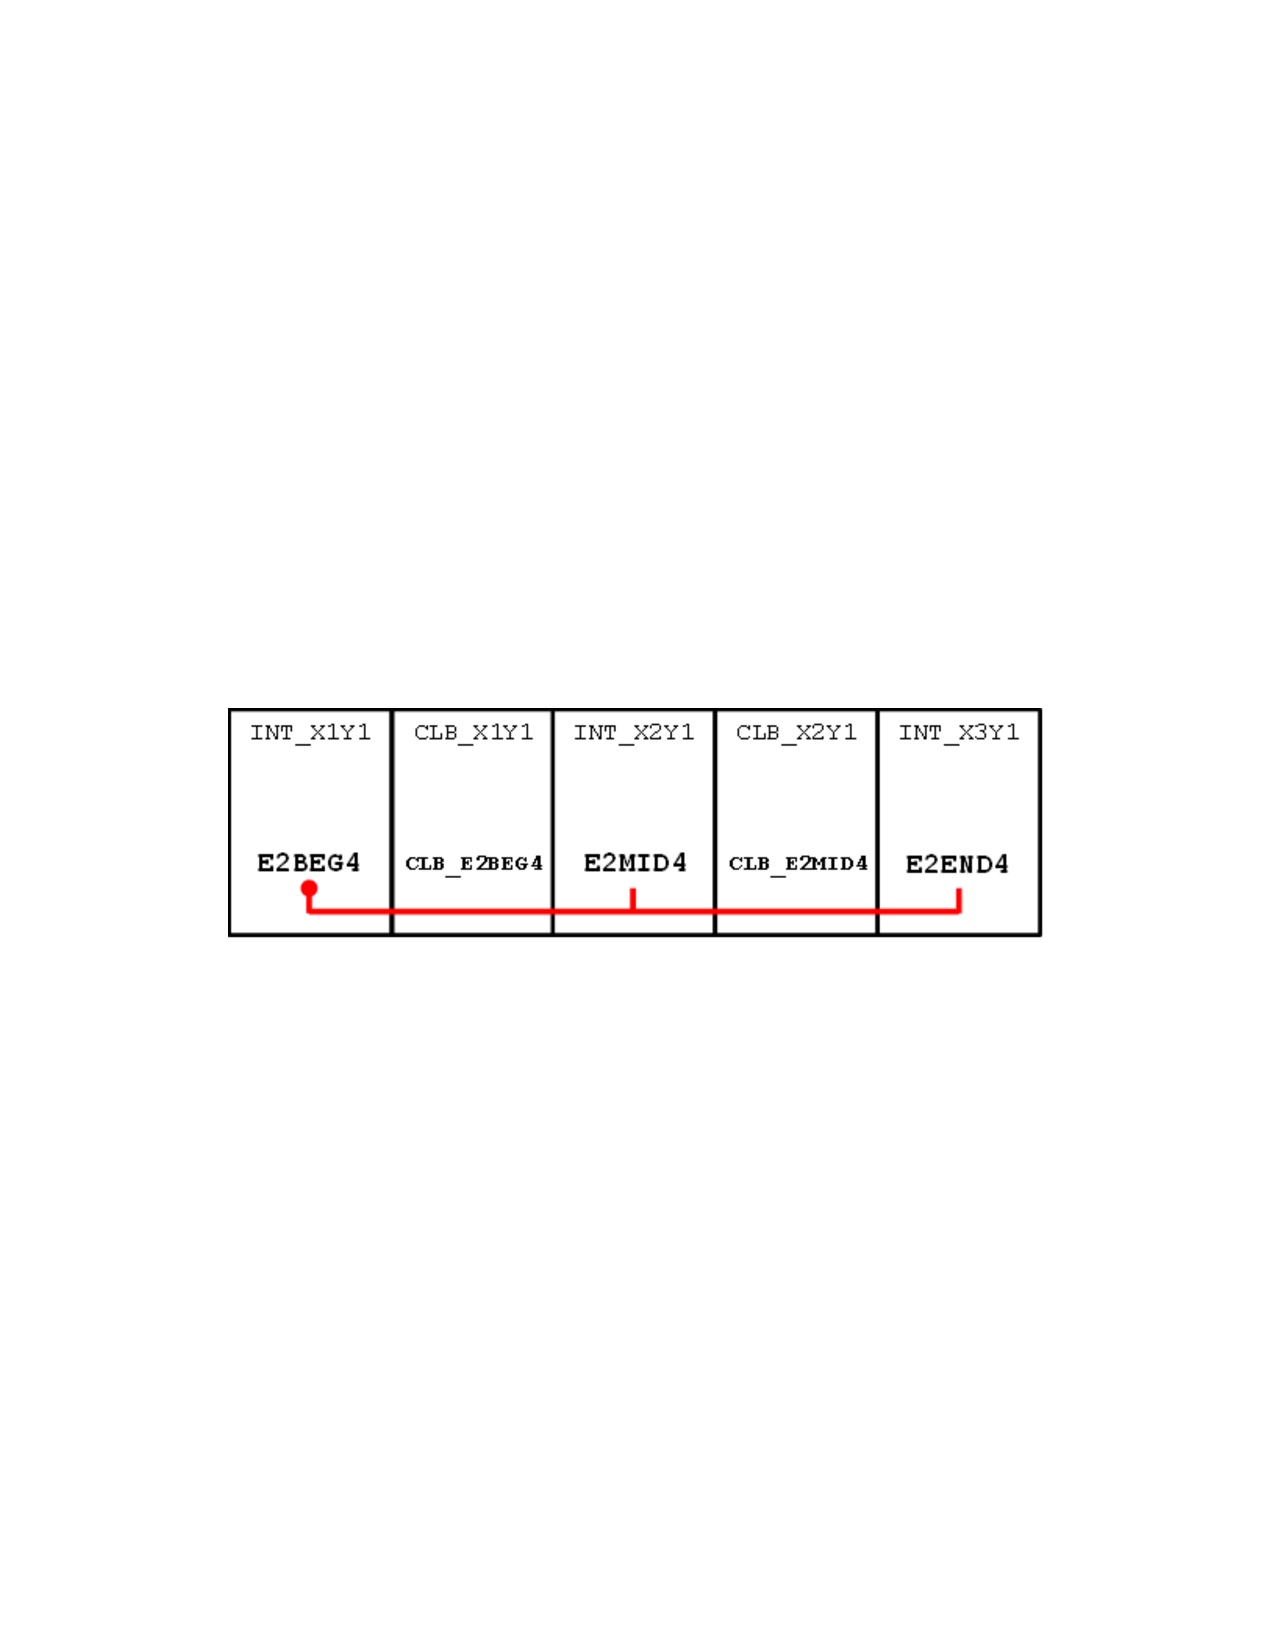
\includegraphics[width=0.8\columnwidth]{wireFigure}
\caption{Multi-Tile Xilinx Wire}
\label{fig:wireFigure}
\end{figure}

\subsection{Traversing Wire Objects}
Traversing through wires in a device is straightforward. Given a handle to a
\texttt{Wire} object named "mywire" or a \texttt{Connection} object named
"conn", the following function calls can be used:

\begin {itemize}
  \item \texttt{mywire.getWireConnections()}: Returns a collection of all
  \texttt{Connection} objects whose source is ``mywire''. This collection can
  be iterated over to find all places a specific wire goes (i.e. what wires it
  connects to).
  \item  \texttt{conn.isPip()}: Returns true if the wire connection ``conn'' is
  a PIP connection. Returns false otherwise.
  \item \texttt{conn.getSinkWire()}: Returns the sink wire of a wire connection.
\end{itemize} 

\noindent
In general, these are the only three functions that are needed to
search through the wires of a FPGA device. It is important to note however that
the first wire in the route must be either (a) created using a \texttt{TileWire}
constructor, or (b) retrieved from a function call of another object (such as
\texttt{SitePin::getExternalWire()}). \autoref{code:connections} demonstrates
how to iterate over \texttt{Connection} objects. To gain a better
understanding of how to use \texttt{Wire}s and \texttt{Connection}s, see the
\textbf{HandRouter} example in the RapidSmith2 repository.

\subsection{Other Types of Connections} \label{otherConns}
Along with PIP and non-PIP wire connections, there are several other types of
connections in RapidSmith2. The source of the connection is always a
\texttt{Wire} object, but the sink object differs. A description of these
connections is found below:

\begin {itemize}
  
  \item \textbf{Site Pin Connections}: Connects a \texttt{Wire} to a
  \texttt{SitePin}. The function call \texttt{Connection::.get\-SitePin()} can
  be used to return a handle to the site pin.
  
  \item \textbf{Terminal Connections}: Connects a \texttt{Wire} to a \texttt{BelPin}. The
  function call \texttt{conn.get\-BelPin()} can be used to return a handle to
  the BEL pin.
  
  \item \textbf{Site Routethrough Connections}: Connects an input site \texttt{Wire}
  to an output site \texttt{Wire}. A \texttt{Site} in Vivado can be configured to pass
  the signal on an input pin directly to an output pin. These connections are
  represented as routethroughs in RapidSmith2 and can be determined with the
  function call \texttt{Connection::isRoutethr\-ough()}.
  \textbf{NOTE}: Before using this type of connection when building a
  routing data structure, make sure the corresponding site is unused.
  
  \item \textbf{BEL Routethrough Connections}: Connects an input BEL \texttt{Wire} to
  an output BEL \texttt{Wire}. LUTs in Vivado can also be configured as
  routethroughs. A BEL routethrough connection can be used while routing the
  inside of a site if there is no cell placed on the
  corresponding BEL.
\end{itemize}

\noindent
When traversing through the device data structure, a generic \texttt{Connection}
object is usually used. This connection can refer to any of the connections
described so far in this documentation. \autoref{code:connections} demonstrates
how to iterate through different \texttt{Connection} types in RapidSmith2.

\begin{lstlisting}[xleftmargin=1.5em, framexleftmargin=1.5em, caption=How to
iterate over Connections in RapidSmith2, label=code:connections] 
  // Get a handle to a wire
  Wire wire = sitePin.getExternalWire();

  // Iterate over all WireConnections
  for (Connection conn : wire.getWireConnections()) {
	  Wire sinkWire = conn.getSinkWire();

	  if (conn.isPip()) {
		  // Do something with a PIP
	  } 
	  else if (conn.isRoutethrough()) {
		  // Do something with a routethrough
	  } 
	  else {	
		  // Do something with a regular wire connection				
	  }
  }

  // Get the site pin connected to a wire
  SitePin pin = wire.getConnectedPin();
  if (pin != null)
	  // Do something with the SitePin
  }

  // Get the bel pin connected to a wire
  BelPin pin = wire.getTerminal();
  if (pin != null)
	  // Do something with the BelPin
  }

  // Iterate over all connections at the same time
  Iterator<Connection> connIt = wire.getAllConnections().iterator();

  while (connIt.hasNext()) {
	  Connection conn = connIt.next();
	
	  if (conn.isPinConnection()) {
		  //do something with the site pin
	  }
	  else if (conn.isTerminal()) {
		  //do something with the bel pin 
	  }
	  else if (conn.isPip()) {
		  //do something with the pip wire connection
	  }
	  else {
		  //do something with regular wire connection.
	  }
  }
\end{lstlisting}

\subsection{RouteTrees}

\texttt{Wire}s and \texttt{WireConnection}s are the fundamental objects used to
specify and explore routing in RapidSmith2, but they need to be organized in
a higher-level data structure to give meaning to the route of a \texttt{CellNet}.
In the original RapidSmith, creating this data structure was up to the user.
RapidSmith2 introduces the \texttt{RouteTree}, which can be seen in
\autoref{fig:routeTreeDS}.

\begin{figure}[H]
\centering
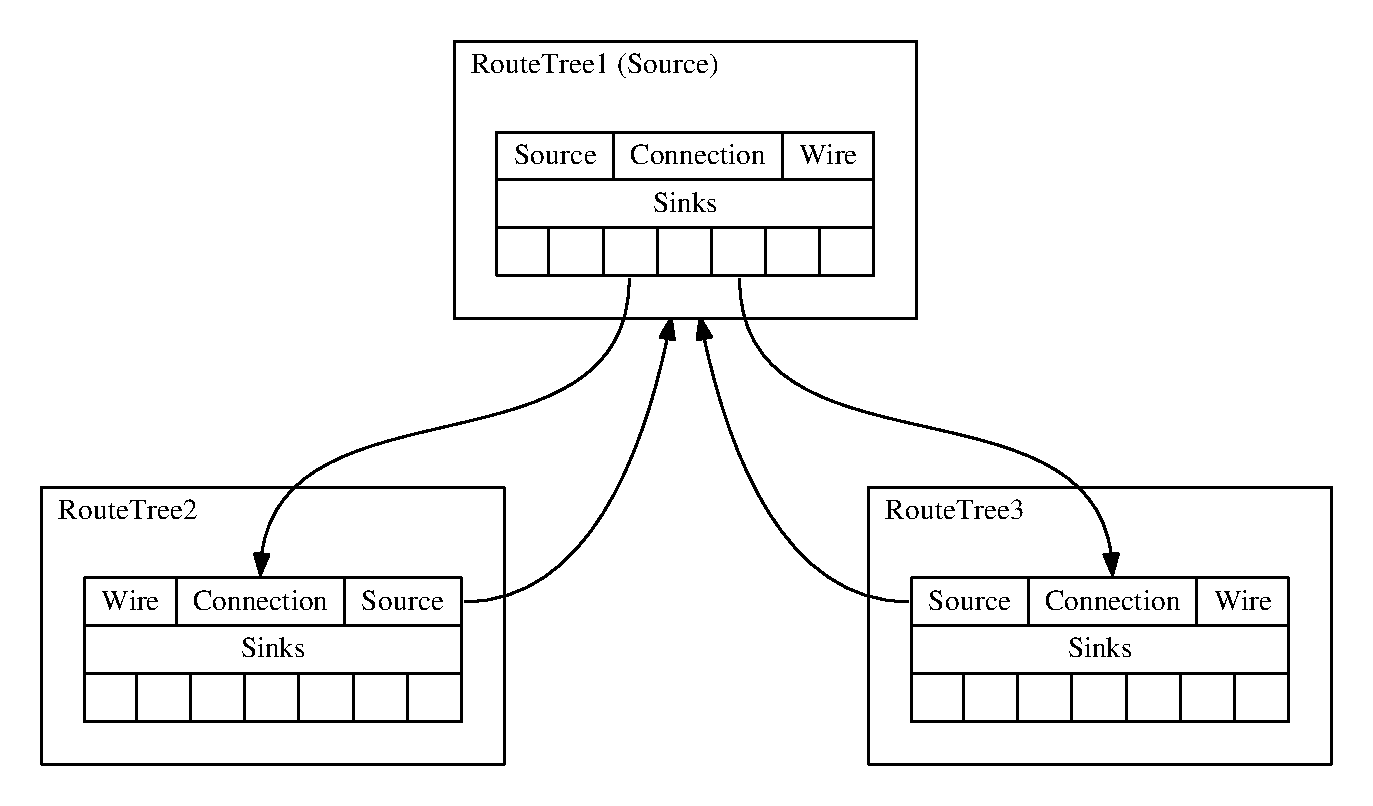
\includegraphics[width=0.8\columnwidth]{routeTreeDS.eps}
\caption{Visual Representation of a RapidSmith2 RouteTree}
\label{fig:routeTreeDS}
\end{figure}

\noindent
As the figure shows, a \texttt{RouteTree} is a simple tree data structure. Each
node in the tree represents a physical wire in the device, and is connected to
other nodes (wires). Edges in the tree represent wire connections (i.e. how one wire
connects to another). A \texttt{RouteTree} can also be conceptually thought of as
a graph, with a single ``starting'' node and several ``sink'' nodes. A
\texttt{RouteTree} node contains the following members:

\begin{figure}[b!]
\centering
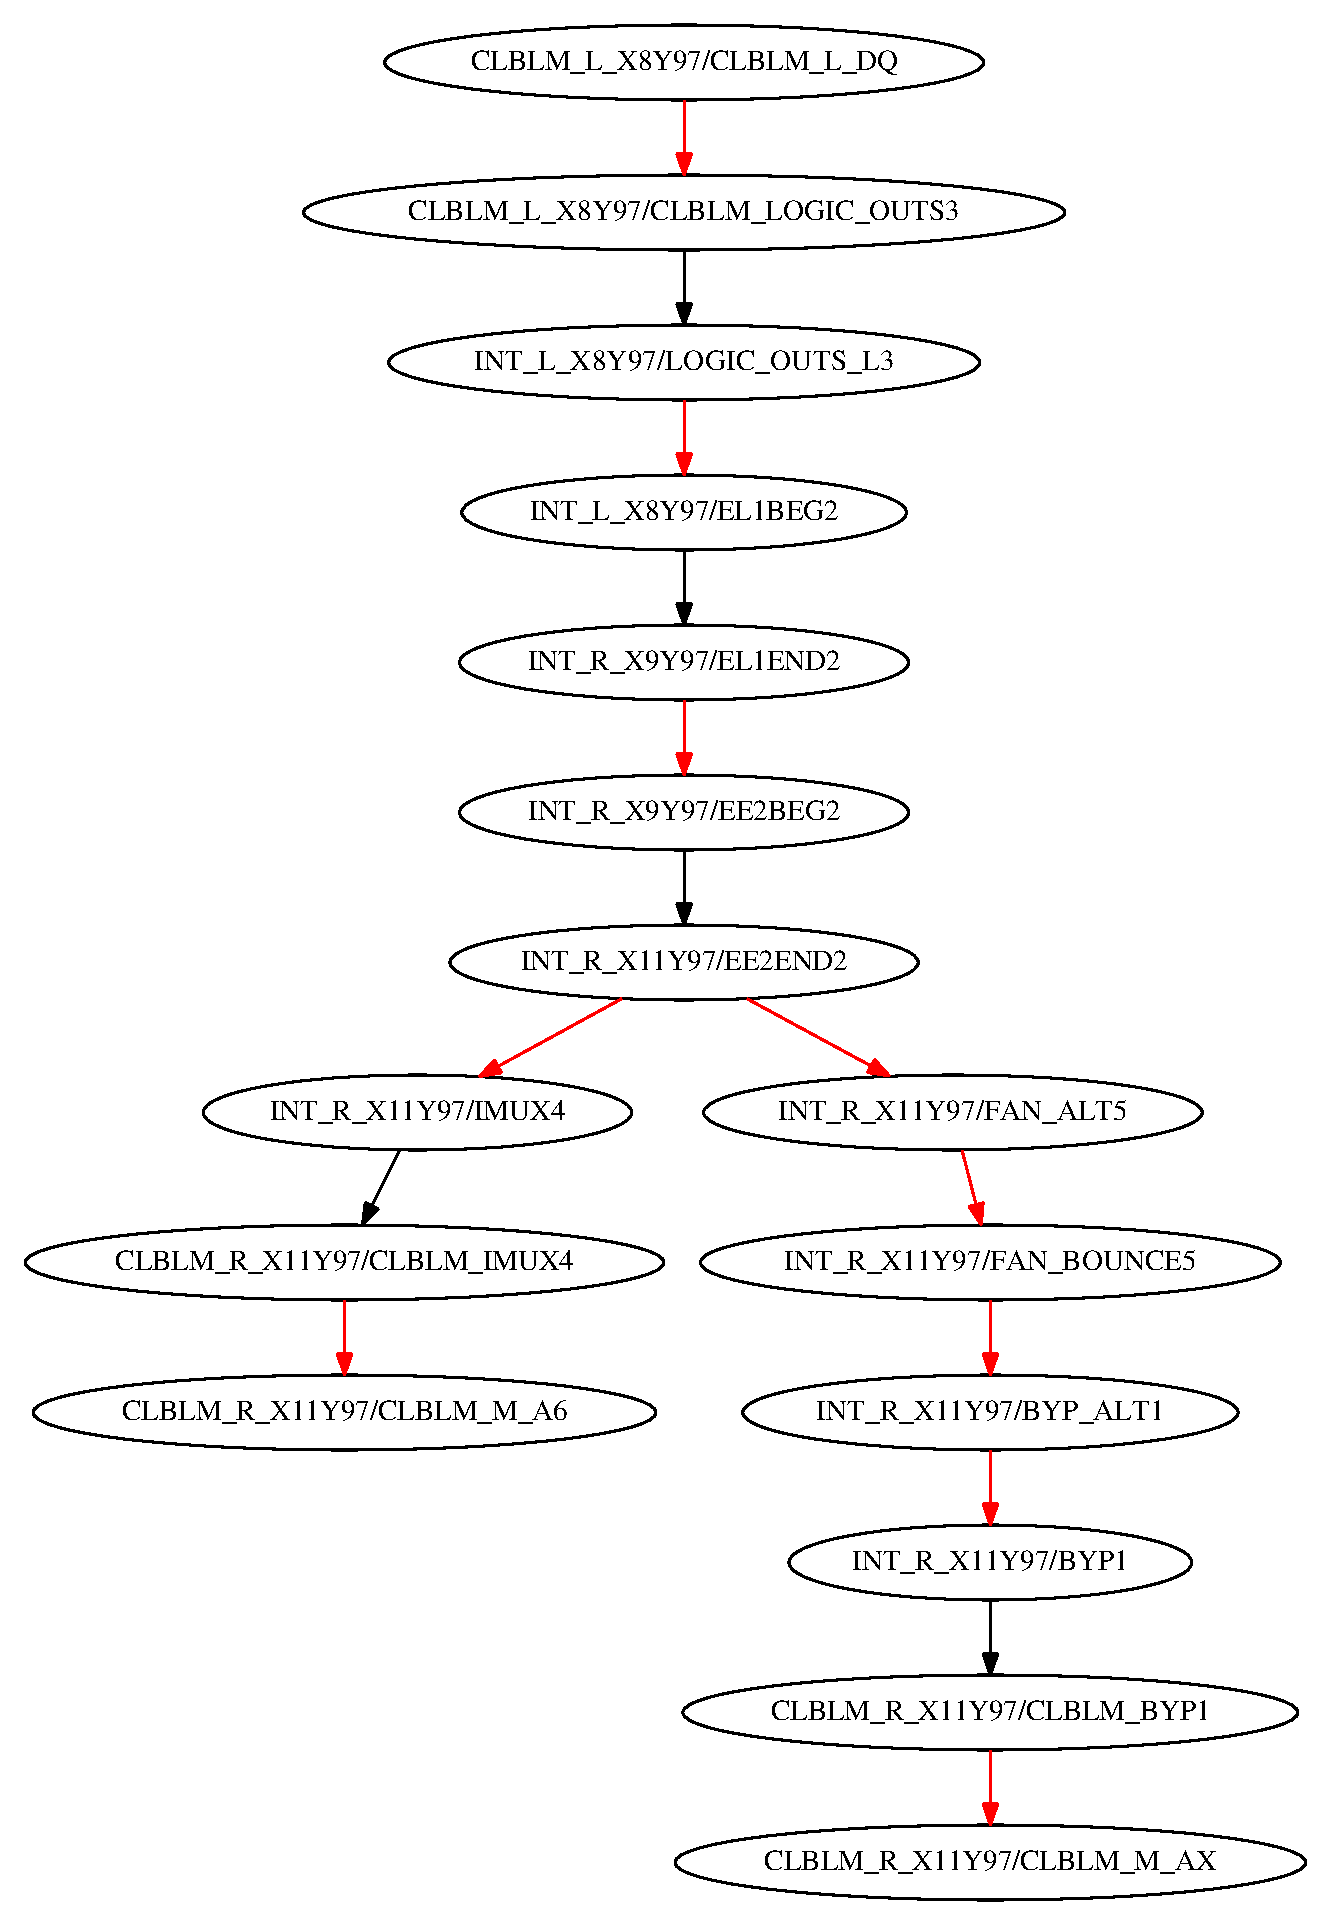
\includegraphics[width=0.65\columnwidth]{routeTree.eps}
\caption{Sample RapidSmith2 RouteTree (red edges represent PIP connections)}
\label{fig:routeTree}
\end{figure}

\begin{itemize}
  \item \textbf{Wire}: The physical \texttt{Wire} object that the \texttt{RouteTree} node
  represents. This can be either a \texttt{TileWire} or \texttt{SiteWire}.
  
  \item \textbf{Source}: A link to the parent \texttt{RouteTree} node
   
  \item \textbf{Connection}: The \texttt{Connection} taken from the \textbf{parent}
  \texttt{RouteTree} node to reach the \textbf{current} \texttt{RouteTree}
  node. In other words, it is the \texttt{Connection} object that was taken
  from the parent wire to reach the current wire.
  
  \item \textbf{Sinks}: A list of child nodes. There is no limit
  to how many children a \texttt{RouteTree} can have.
  
  \item \textbf{Cost} (not shown): An optional cost field for routers 
\end{itemize}

A complete \texttt{RouteTree} specifies how the source of a
\texttt{CellNet} is physically connected to all of its sinks.
\autoref{fig:routeTree} shows an example of a complete \texttt{RouteTree} in
RapidSmith2. As can be seen, the \texttt{CellNet} that is being routed has once
source site pin, and two sink site pins. The source pin is connected to wire
\texttt{CLBLM\_L\_X8Y97/CLBLM\_L\_DQ}, and the sink pins are connected to the
wires \texttt{CLBLM\_R\_X1Y97/CLBLM\-\_M\_A6} and
\texttt{CLBLM\-\_R\_X11Y97/CLBLM\_M\_AX}. Starting from the source, wires are
traversed downward (via wire connections) until the target wires are reached.
\autoref{code:routeTree} demonstrates the basic usage of \texttt{RouteTree}s in
RapidSmith2. The \textbf{DesignAnalyzer}, \textbf{AStarRouter}, and
\textbf{HandRouter} examples in the RapidSmith2 repository also demonstrate
how to traverse and build a \texttt{RouteTree}.

\begin{lstlisting}[xleftmargin=1.5em, framexleftmargin=1.5em, caption=Building a
RouteTree, label=code:routeTree] 
  // Find a Wire to start the RouteTree at
  Site site = device.getSite("SLICE_X5Y84");
  SitePin pin = site.getSitePin("DQ");
  Wire startWire = sink.getExternalWire();

  // Create the first node in the RouteTree 
  Queue<RouteTree> rtQueue = new LinkedList<RouteTree>();
  RouteTree start = new RouteTree(startWire);
  rtQueue.add(start);

  // Build up the RouteTree somehow 
  while (!amDone()) {
	  RouteTree current = rtQueue.poll();
	  Wire wire = route.getWire();

	  for (Connection conn : wire.getWireConnections()) {
		  // add qualified connections to the RouteTree
		  if (isQualified(wire)) {
			  RouteTree tmp = current.addConnection(conn);
			  rtQueue.add(tmp);
		  }
	  }
  }
\end{lstlisting}

When a design is imported from Vivado through a RSCP, the routing information
is parsed and loaded into \texttt{Route\-Tree}s for each \texttt{CellNet}. On
design export, the \texttt{RouteTree} for each \texttt{CellNet} is traversed
and converted into a Vivado \texttt{ROUTE} string. Users can use custom data
structures to route a design, but they need to be \textbf{converted to an
equivalent RouteTree representation} before exporting the design to Vivado.  

\subsection{Three Part Routing} \label{sec:threePartRouting}
In RapidSmith2, there are three sections to a routed \texttt{CellNet}: 

\begin{enumerate}
  \item The portion of the net that starts at the source BEL pin, and is routed
  to an output site pin. This part of the route exists completely inside of
  site boundaries.
  
  \item The portion of the net that starts at the output site pin of part (1),
  and is routed to several sink site pins. This part of the route is
  called the \textbf{intersite} route because it connects sites together. A
  typical router is responsible for routing this section of the
  net\footnote{VCC and GND nets don't follow this pattern. The main difference
  for VCC and GND is that they can have multiple intersite nets.}.
  
  \item The portion of the net that starts at the sink site pins from part (2),
  and is routed to sink BEL pins. Since there can be several sink pins in a
  \texttt{CellNet}, this section of the net can have more than one component.
  Each component exists completely inside site boundaries.
\end{enumerate}

\noindent \autoref{fig:threePartRouting} shows a visual representation of the
three-part routing structure. Each section of a route has a corresponding
\texttt{RouteTree} object. A source \texttt{RouteTree} represents the orange
wires in the figure (part 1), an intersite \texttt{RouteTree} represents the
green wires in the figure (part 2), and a list of sink \texttt{RouteTree}s
represents the purple wires in the figure (part 3, with a different
\texttt{RouteTree} object for each site). It is important to note that
intrasite nets only have a source \texttt{RouteTree} because they are
completely contained within a site. \autoref{code:threePartRouting} demonstrates
how to utilize three-part routing in RapidSmith2. On design import, the routing
sections of each \texttt{CellNet} are created automatically.

\begin{figure}[t]
\centering
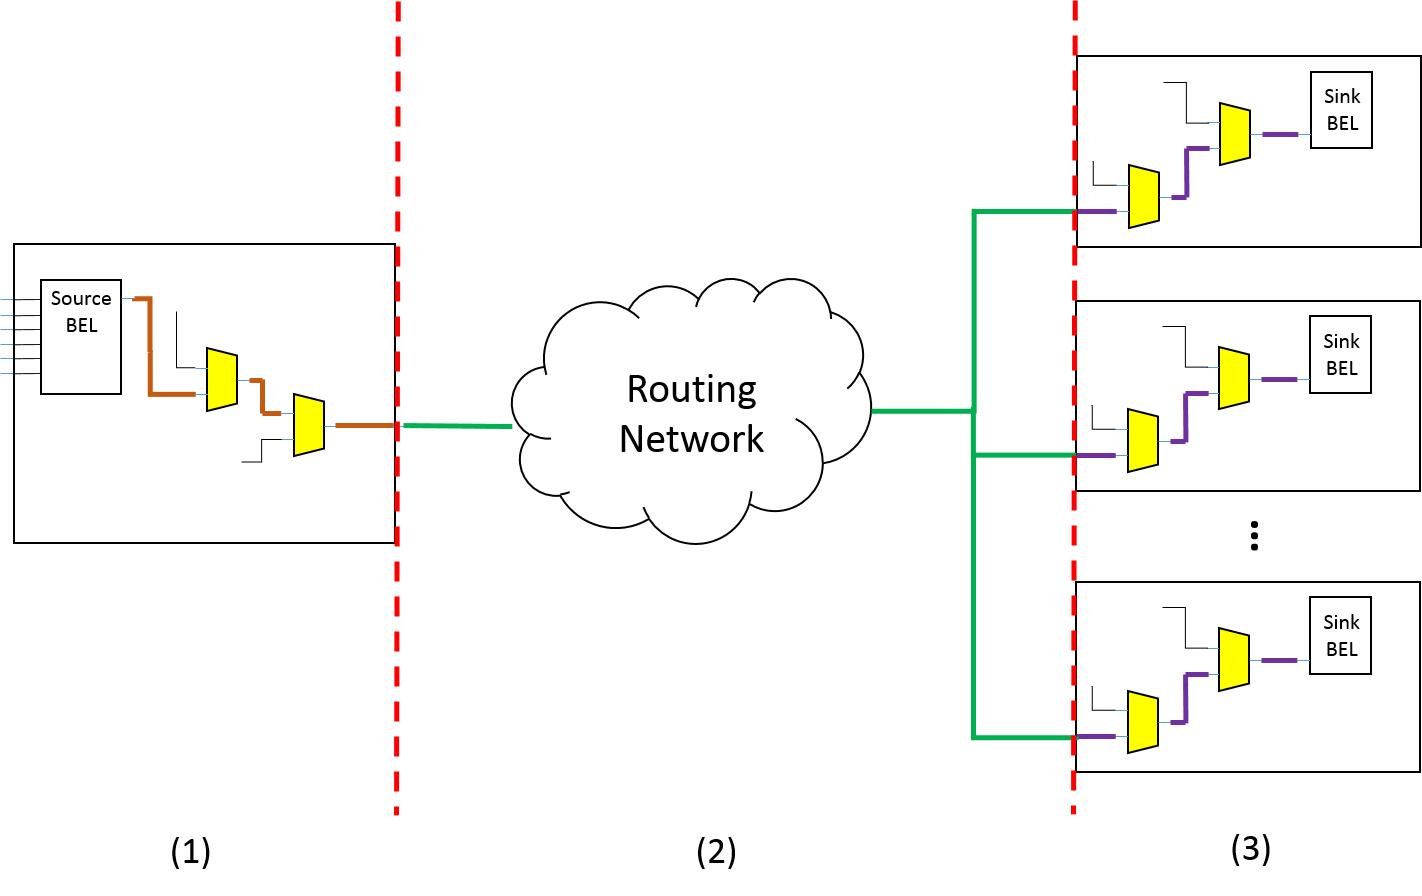
\includegraphics[width=1\columnwidth]{threePartRouting.png}
\caption{Three-Part Routing}
\label{fig:threePartRouting}
\end{figure}

\begin{lstlisting}[xleftmargin=1.5em, framexleftmargin=1.5em,
caption=Demonstration of three-part routing in RapidSmith2,
label=code:threePartRouting] 
  // Get a handle to a routed net in the design 
  CellNet net = design.getNet("myNet");

  // Handling the source RouteTree
  RouteTree source = net.getSourceRouteTree();
  net.setSourceRouteTree(createSourceRoute());

  // Handling the intersite RouteTree
  RouteTree intersite = net.getIntersiteRouteTree();
  net.addIntersiteRouteTree(createIntersiteRoute());

  // Iterate over a list of sink RouteTrees
  for (RouteTree rt : net.getSinkSitePinRouteTrees()) {
	  // do something with the RouteTree
  }

  // Or, get a RouteTree based on a SitePin
  for(SitePin sitePin : net.getSitePins()) {
	  if (sitePin.isInput()) {
		  RouteTree sinkTree = net.getSinkTree(sitePin);
		  // do something with the RouteTree
	  }
  }

  // Add a new sink RouteTree that starts at a SitePin
  net.addSinkRouteTree(sitePin, createSinkRouteTree(sp));
\end{lstlisting}


\subsection{Routing in Vivado}
The reason a three-part routing distinction is necessary in RapidSmith2, is due
to how routing is represented in Vivado. Inside site boundaries, a route is
represented using site PIPs. A string of enabled PIPs determines what pins
are connected together within the site. Between site boundaries, a route is
instead represented using wires. The wires are formatted into a Vivado ROUTE
string, which uniquely specifies the intersite route for a net. The three-part
routing representation makes this distinction explicit to the users of
RapidSmith (it also makes import/export easier). When a design is exported from
Vivado, the intrasite portions of a net are exported as site PIPs, and the
intersite portion of the net is exported as wires.

\begin{lstlisting}[numbers=none, keywordstyle=, stringstyle=]
// An example of a string of used site pips in Vivado
{IUSED:0 IBUFDISABLE_SEL:GND INTERMDISABLE_SEL:GND}

// An example of a Vivado ROUTE string
 { CLBLL_LL_AQ CLBLL_LOGIC_OUTS4  { NW6BEG0 NE2BEG0 WR1BEG1 IMUX_L34
IOI_OLOGIC0_D1 LIOI_OLOGIC0_OQ LIOI_O0 }  IMUX_L1 CLBLL_LL_A3 }
\end{lstlisting}

\subsection{Intrasite Routing}
On design import, the site PIP information extracted from Vivado is stored
into RapidSmith2 data structures, and used to reconstruct the three-part
routing view described in the previous section. This gives the user two options
when dealing with intrasite routing in RapidSmith2: (1) use the three-part
routing data structures, or (2) use the set of enabled site PIPs stored in the
\texttt{CellDesign}. It is user preference for which representation to use
when writing a CAD tool, but both representations need to be up-to-date before
design export. \autoref{code:sitePips} demonstrates how a set of used site PIPs
can be created and added to a site. This step needs to be taken \textbf{only
when you have modified the intrasite routing} for a site.

\begin{lstlisting}[xleftmargin=1.5em, framexleftmargin=1.5em, caption=Code
to transform a set of SiteWires into Site PIPs, label=code:sitePips]
  // Get a handle to a Design and a Site
  CellDesign design = vcp.getDesign();
  Device device = vcp.getDevice();
  Site site = device.getSite("SLICE_X5Y84");

  // Get a list of used site wires somehow (this is up to you)
  Set<Wire> usedSiteWires = getUsedWires(site);

  // Convert the list of wires to their integer enumeration
  Set<Integer> usedPipWires = usedSiteWires.stream()
										 .map(w -> w.getWireEnum())
										 .collect(Collectors.toSet());

  // Set the used site pips with the design class
  design.setUsedSitePipsAtSite(site, usedPipWires);
\end{lstlisting}
